% Latex template: mahmoud.s.fahmy@students.kasralainy.edu.eg
% For more details: https://www.sharelatex.com/learn/Beamer

\documentclass{beamer}					% Document class

\usepackage[portuguese]{babel}				% Set language
\usepackage[utf8x]{inputenc}			% Set encoding

\mode<presentation>						% Set options
{
  \usetheme{default}					% Set theme
  \usecolortheme{default} 				% Set colors
  \usefonttheme{default}  				% Set font theme
  \setbeamertemplate{caption}[numbered]	% Set caption to be numbered
}

\setbeamertemplate{navigation symbols}{}
\setbeamertemplate{footline}[frame number]
\setbeamercovered{transparent}

% Uncomment this to have the outline at the beginning of each section highlighted.
%\AtBeginSection[]
%{
%  \begin{frame}{Outline}
%    \tableofcontents[currentsection]
%  \end{frame}
%}

\usepackage{graphicx}					% For including figures
\usepackage{booktabs}					% For table rules
\usepackage{hyperref}					% For cross-referencing

\title{Revisão de Atividades da FAC}	% Presentation title
%\author{Author One}								% Presentation author
\institute{LNLS.DAC.FAC}					% Author affiliation
\date{2023-09-22 -- 2023-10-06}									% Today's date	

\begin{document}

% Title page
% This page includes the informations defined earlier including title, author/s, affiliation/s and the date
\begin{frame}
  \titlepage
  \href{https://github.com/lnls-fac/doc-review-dac-fac}{\beamergotobutton{Link para o repo github desta apresentação: https://github.com/lnls-fac/doc-review-dac-fac}}
  \href{https://www.overleaf.com/read/sbdjxtzfchrm}{\beamergotobutton{Link para o projeto overleaf destas notas}}
  
  
\end{frame}

% Outline
% This page includes the outline (Table of content) of the presentation. All sections and subsections will appear in the outline by default.
\begin{frame}{Outline}
  \tableofcontents
\end{frame}

% The following is the most frequently used slide types in beamer
% The slide structure is as follows:
%
%\begin{frame}{<slide-title>}
%	<content>
%\end{frame}


\section{Estudos de máquina - 25/09 Instabilidade longitudinal CB}


\begin{frame}{25/09 Instabilidade longitudinal CB}

    \begin{itemize}
		\item Usamos este turno de experimento para entender a questão da instabilidade longitudianl após a troca de canal de sinal no LLRF.
	\end{itemize}

    \begin{figure}[H]
		\centering
        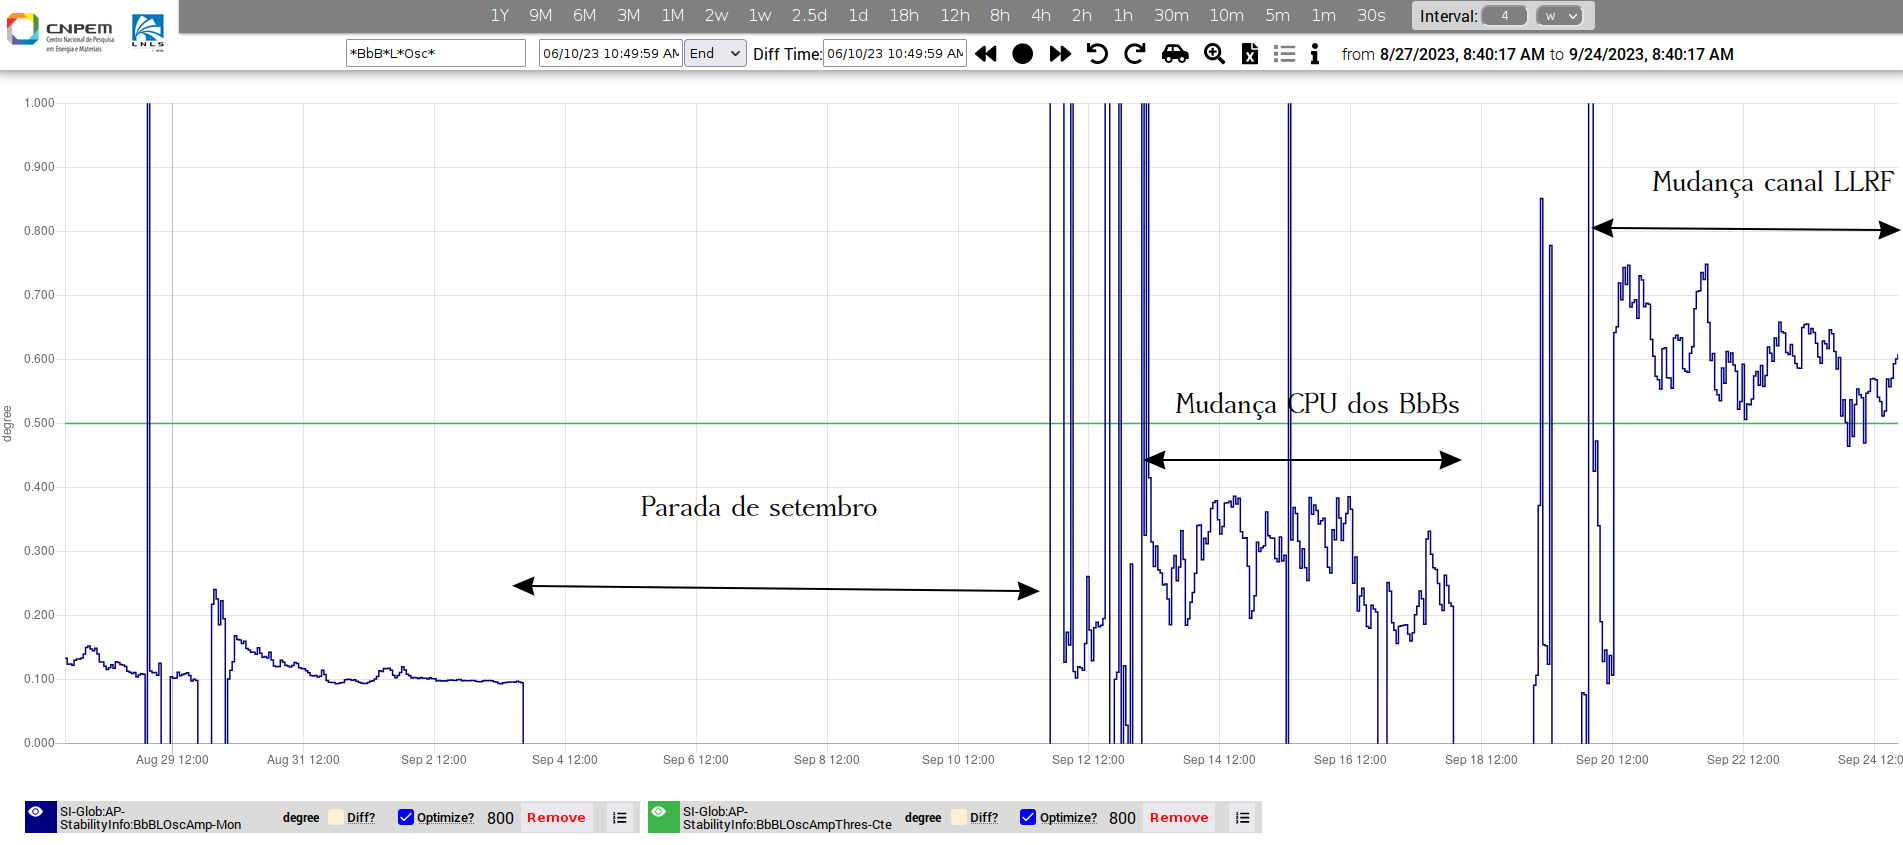
\includegraphics[width=.9\textwidth]{figures/long-osc-before-correction.png}
        \caption{Longitudinal Oscillations (before correction)}
        \label{fig:figure1}
    \end{figure}
    
\end{frame}



\begin{frame}{25/09 Instabilidade longitudinal CB}
    \begin{itemize}
        \item maior oscilação longitudinal no feixe após troca de canal de sinal no LLRF. além disto com ganho diferente do canal a tensão de referência que gera a mesma tensão de aceleração: 308 mV $\rightarrow$ 506 mV para gerar $V_\mathrm{gap} \approx 1.7$ MV.
        \item os parâmetros de PI foram reduzidos em $\sim$ 30\% para compensar a nova tensão de referência 30\% maior. Um pequeno aumento na tensão de gap foi feito para afastar a freq. síncrotron para longe de múltiplos de ``64'' Hz.
        \item procedimento de reconfiguração dos parâmetros do sistema bunch-by-bunch (BbB), participação do grupo de RF
	\end{itemize}
\end{frame}



\begin{frame}{25/09 Instabilidade longitudinal CB}

    \begin{figure}[H]
		\centering
        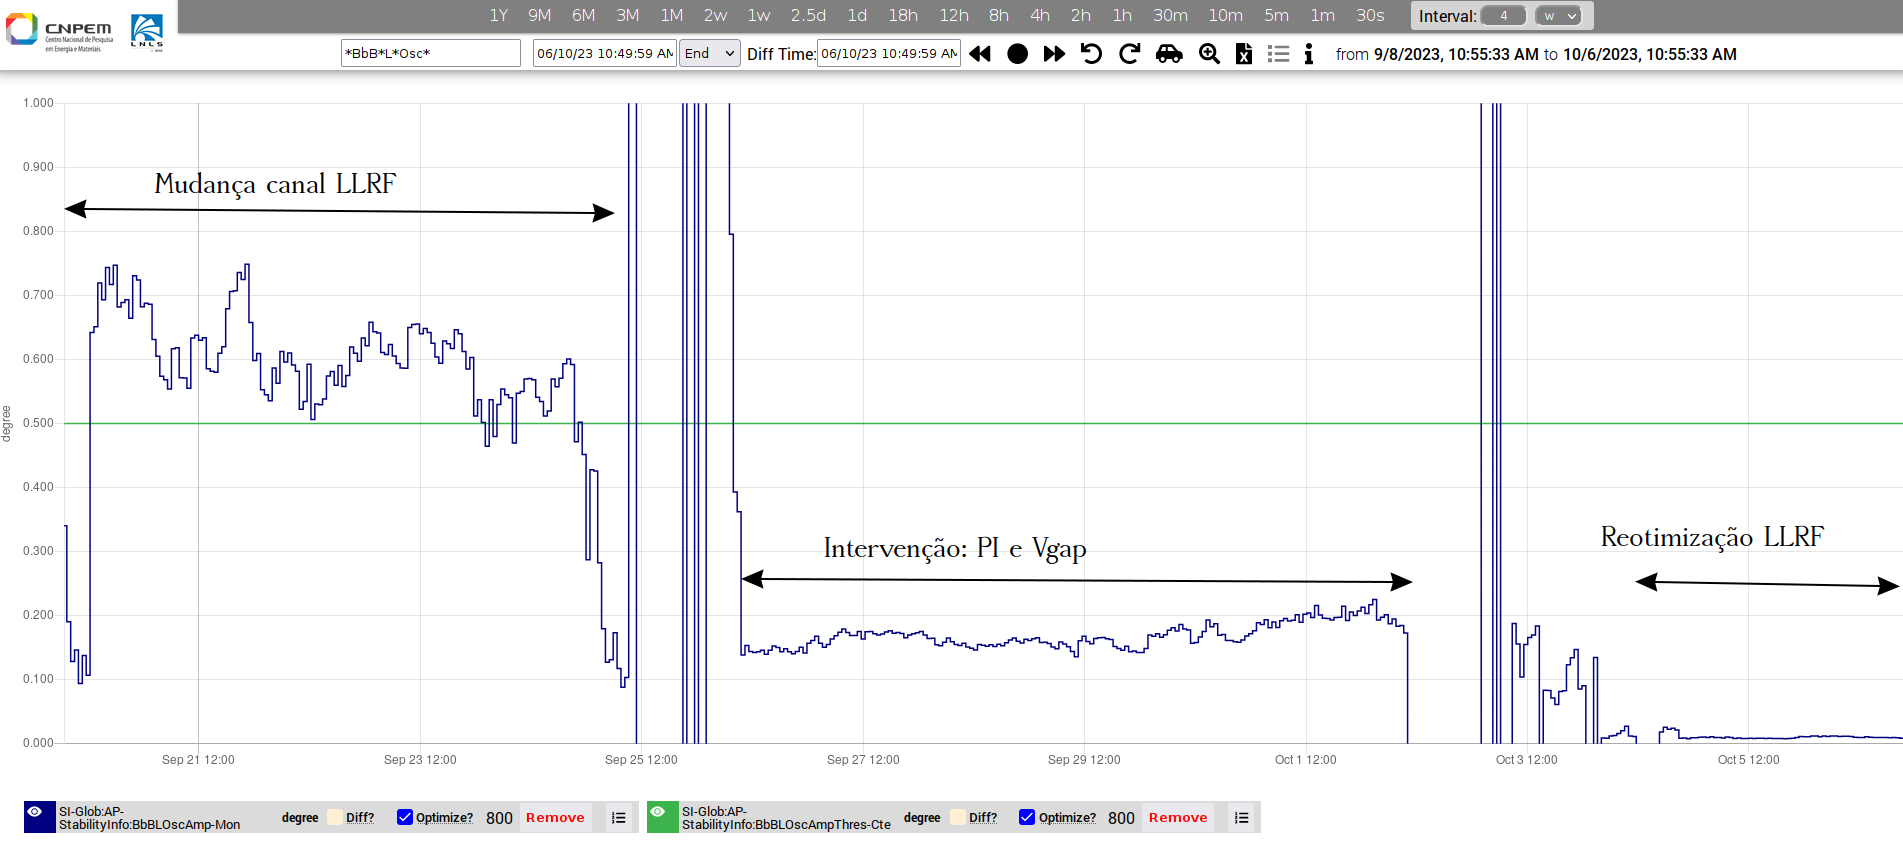
\includegraphics[width=.9\textwidth]{figures/long-osc-after-correction.png}
        \caption{Longitudinal Oscillations (after correction)}
        \label{fig:figure1}
    \end{figure}
    
\end{frame}

\section{Participação no estudo de máquina - 02/10 Otimização LLRF da P7Cav}

\begin{frame}{02/10 Otimização LLRF da P7Cav}

    \begin{itemize}
        \item Ajuste phase shifter $\to$ aumento margem de fase
		\item Reconfiguração de parâmetros PI do LLRF da P7Cav: \newline 
        $K_p: 2 \to 5$, $K_i: 21 \to 5000$
	\end{itemize}

    \begin{figure}[H]
		\centering
        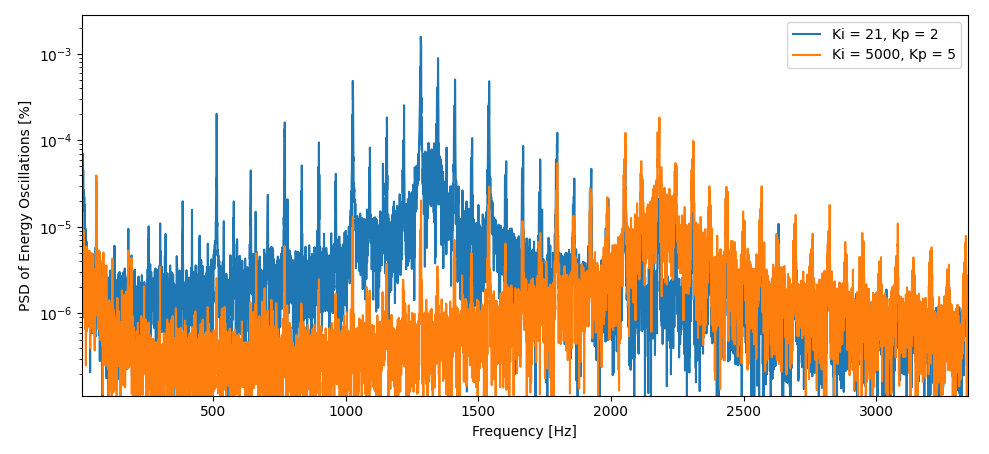
\includegraphics[width=.9\textwidth]{figures/llrf-energy-oscillations.png}
        \caption{Beam oscillation - PSD of energy}
        \label{fig:figure1}
    \end{figure}

\end{frame}



\begin{frame}{02/10 Otimização LLRF da P7Cav}

\begin{itemize}
		\item Redução $\sim$ 8x
\end{itemize}
 
\begin{figure}[H]
		\centering
        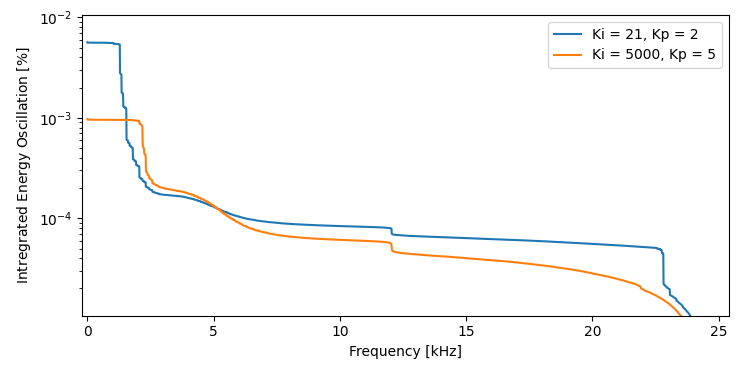
\includegraphics[width=.9\textwidth]{figures/llrf-integrated-energy-oscillations.png}
        \caption{Beam oscillation - Integrated PSD of energy}
        \label{fig:figure1}
\end{figure}

\end{frame}



\begin{frame}{02/10 Otimização LLRF da P7Cav}

\begin{itemize}
		\item Redução $\sim$ 10x
\end{itemize}

\begin{figure}[H]
		\centering
        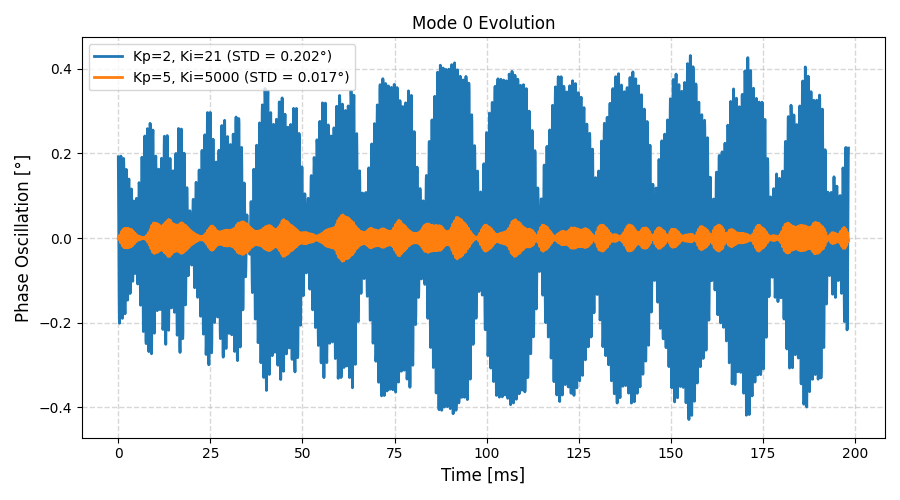
\includegraphics[width=.9\textwidth]{figures/llrf-phase-oscillations.png}
        \caption{Beam oscillation - Phase}
        \label{fig:figure1}
\end{figure}

\end{frame}
 


\section{Estudos de máquina - 03/10 Ajuste da função dispersão}

\begin{frame}{03/10 Ajuste da função dispersão}
    \begin{itemize}
		\item Usando a matrix resposta $\frac{\Delta \eta_y}{\Delta K_sL}$ do modelo nominal atuamos nos skew quads e minimizamos a função dispersão vertical. Redução $\sim$ 5x de $\eta_y$ rms.
    \begin{figure}[H]
		\centering
        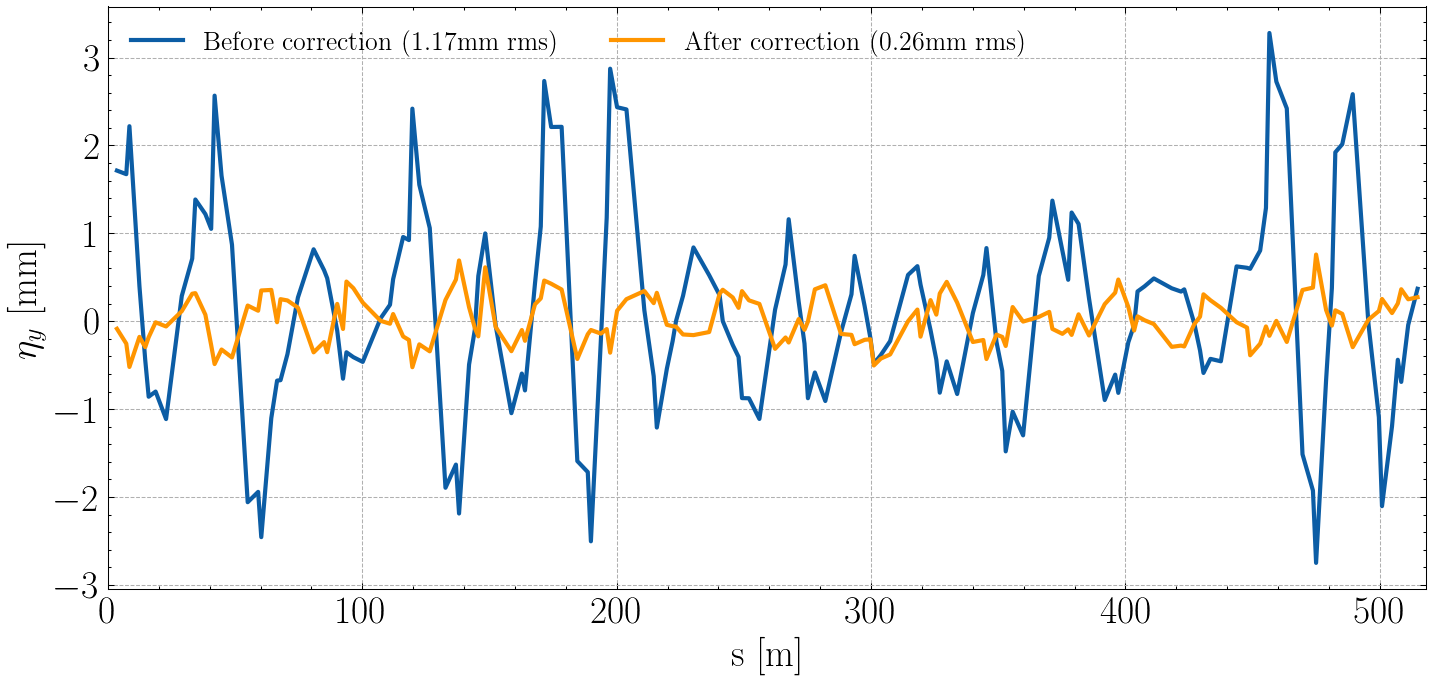
\includegraphics[width=.7\textwidth]{2023-10-06/figures/vertical_dispersion_correction.png}
        % \caption{Dispersão vertical antes e após correção.}
        \label{fig:figure1}
    \end{figure}
    
        \item Medimos acoplamento global $\sim$ 2.6\% e corrigimos com os botões de acoplamento tradicionais para $\sim$ 1.4\% (mínimo possível nessa config.). Ref. config. opera com 1\%.
        \item Tamanho vertical e ângulo maiores na CARCARA com essa config. continuação do estudo em 17/10...
	\end{itemize}
\end{frame}



\section{Atividades - Sinal em 89 Hz observado na Carnaúba 06SB}

\begin{frame}{Sinal em $\sim$ 89 Hz observado na Carnaúba 06SB}
    
    \begin{itemize}
		\item Sinais de corrente ``ai0'' e ``ai1'': pico recente em $\sim$ 89Hz do espectro, maior que o pico em 60Hz, que já existia.
        \item Amostragem em 2kHz
	\end{itemize}

    \begin{figure}[H]
		\centering
        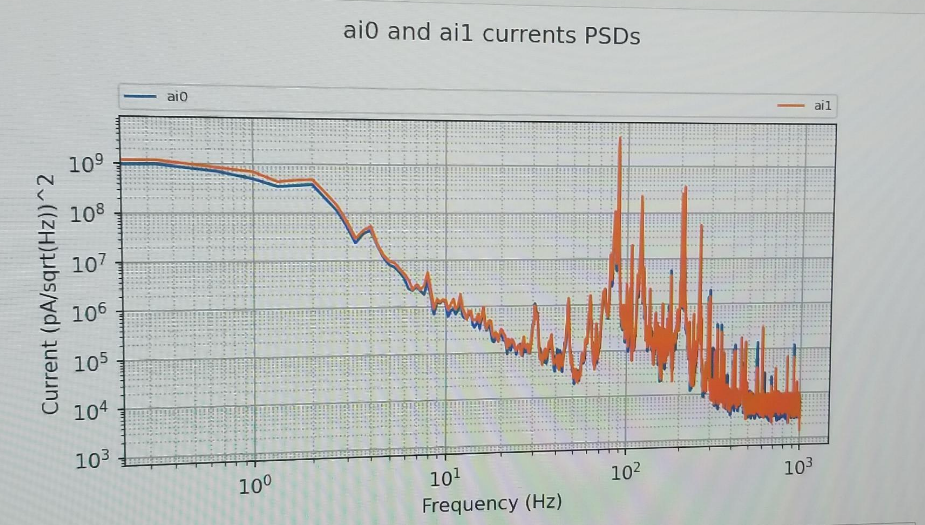
\includegraphics[width=.6\textwidth]{figures/carnauba-89hz-signal.png}
        \caption{PSD do sinal do feixe de fótons na Carnaúba}
        \label{fig:figure1}
    \end{figure}
    
\end{frame}



\begin{frame}{Estabilidade do feixe de elétrons no centro do trecho 06SB}
    
    \begin{itemize}
		\item Aquisição de órbita BPMs na taxa FOFB (45kHz)
        \item Existe um pico em $\sim$ 89Hz na posição $x$ mas a amplitude é 20 nm rms, 7x menor que pico em 60 Hz com 150 nm rms.
	\end{itemize}

    \begin{figure}[H]
		\centering
        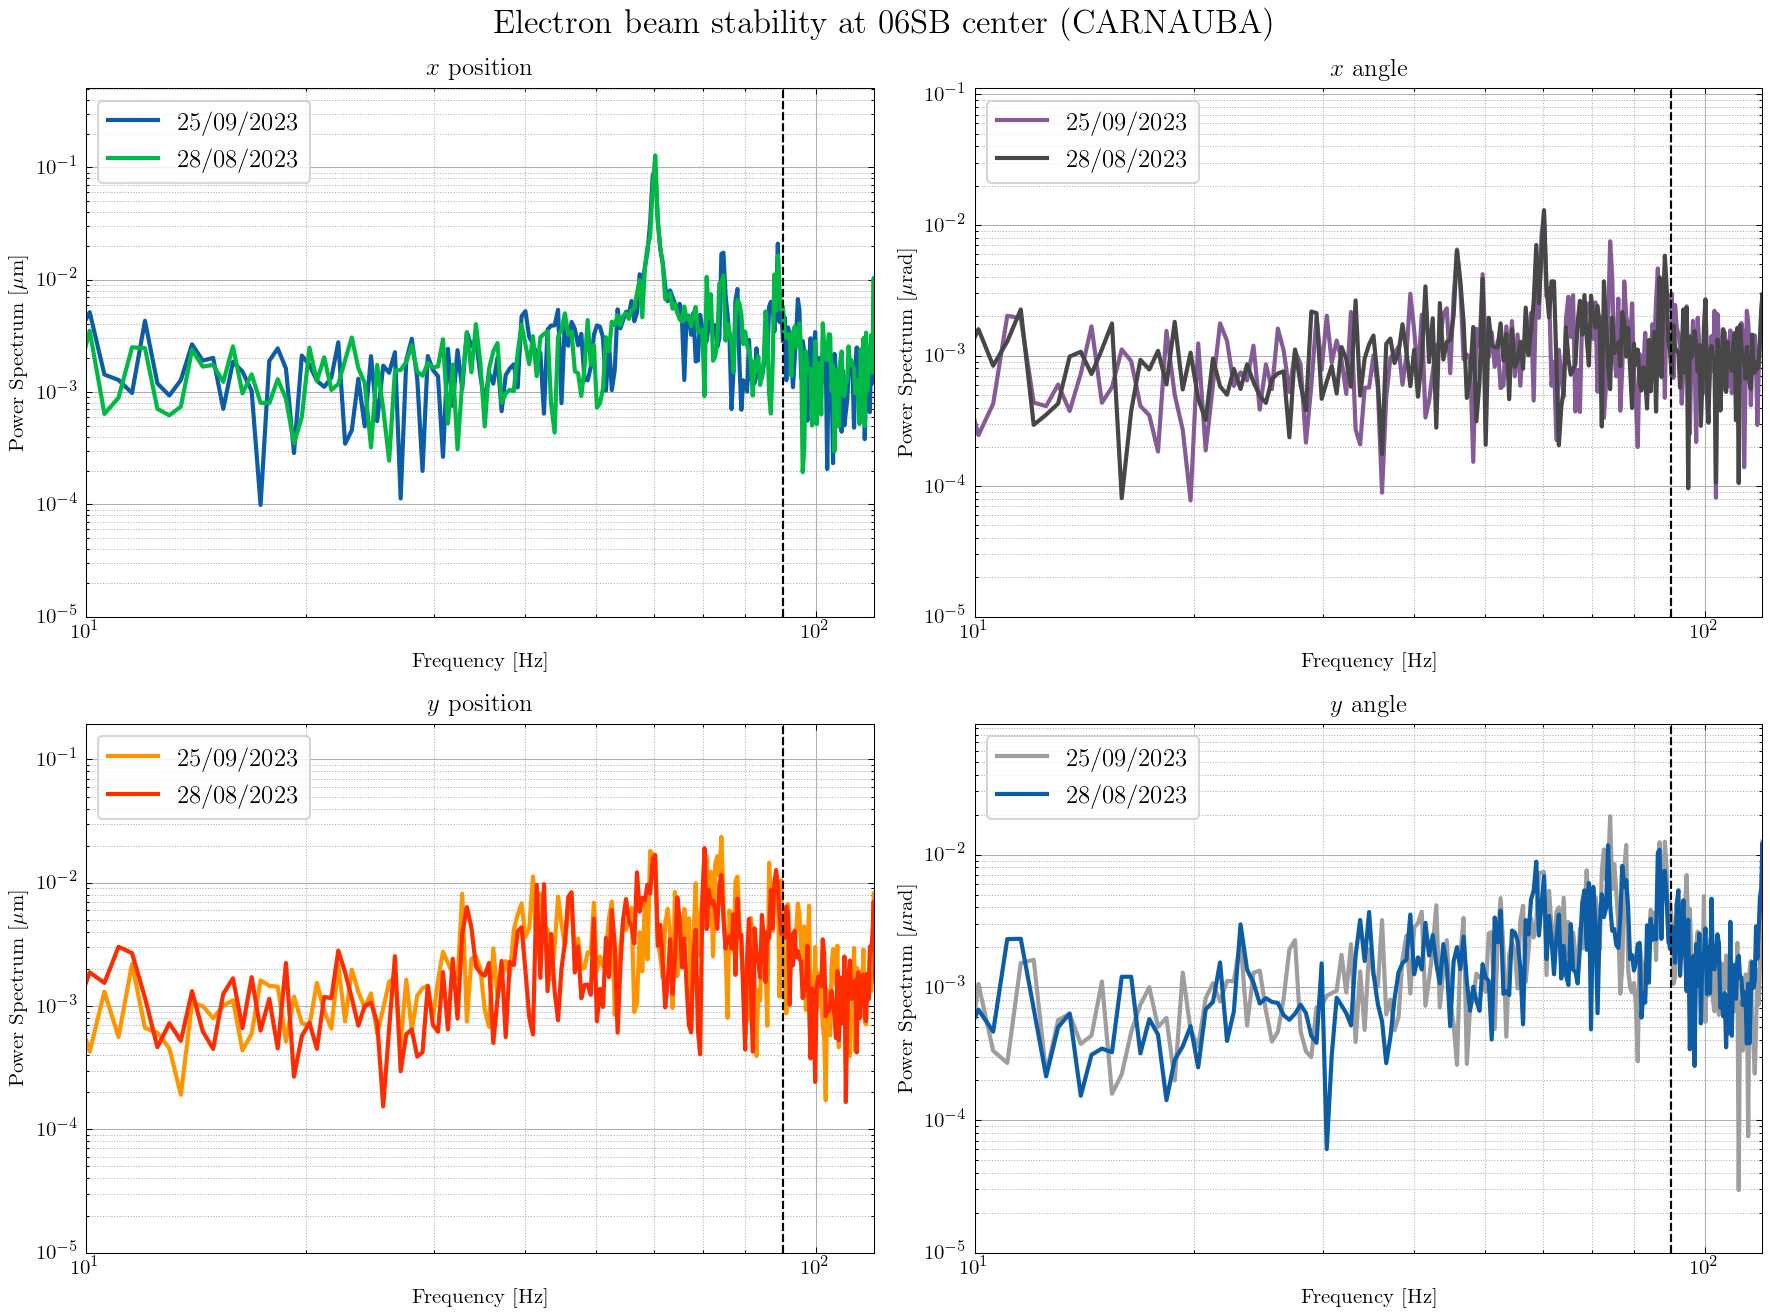
\includegraphics[width=.7\textwidth]{2023-10-06/figures/beam_stability_carnauba_compare_zoom_freqs.png}
        \caption{PSD de posição e ângulo $(x, y)$ no centro do trecho 06SB}
        \label{fig:figure1}
    \end{figure}
    
\end{frame}



\begin{frame}{Estabilidade do feixe de elétrons no centro do trecho 06SB}
    
    \begin{itemize}
		\item Mais medidas deste tipo serão realizadas na Carnaúba, em princípio nos dias 24 e 25 de Outubro. 
        \item Planejamos fazer aquisições trigueradas da órbita concomitantemente para análises.
	\end{itemize}
    
\end{frame}



\section{Atividades - Calibração modelo RADIA do DELTA52}

\begin{frame}{Calibração modelo RADIA do DELTA52}
    \begin{itemize}
		\item A ideia é ter um modelo RADIA 3D do ID que explique as medidas de mapas de campo feitas com sensor Hall, que no caso do DELTA, só podem ser feitas no plano $y = 0$. Com este modelo calibrado podemos fazer RK para resolver a traj. 3D e obter os mapas de kicks transversais $x'(x_0, y_0)$ e $y'(x_0, y_0)$ para estudar o efeito do ID na ótica e abertura dinâmica.
        \item Usando as medidas de mapas de campo com sensor Hall, calibramos o modelo RADIA do ID (sem magic finger)
	\end{itemize}
\end{frame}

\begin{frame}{Calibração modelo RADIA do DELTA52}
\begin{itemize}
        \item Fitting de campo de um modelo DELTA52 com magnetizações aleatórias.
	\end{itemize}
\begin{figure}[H]
		\centering
        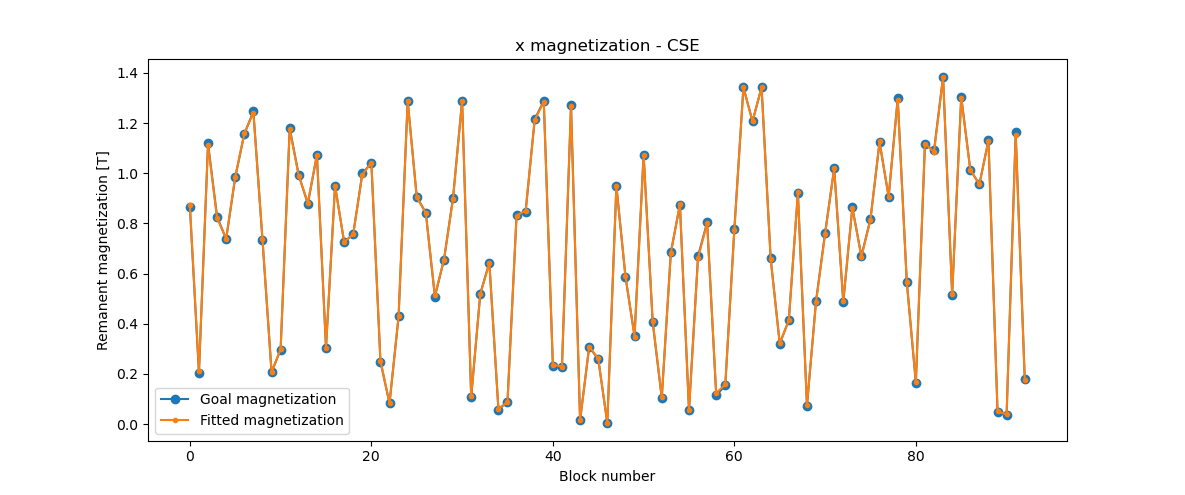
\includegraphics[width=.9\textwidth]{figures/mag_fitting.png}
        \caption{Comparação entre magnetizações encontradas pelo algoritmo e magnetizações objetivo.}
        \label{fig:mag_fitting}
    \end{figure}
\end{frame}

\begin{frame}{Calibração modelo RADIA do DELTA52}
\begin{itemize}
        \item Fitting de medidas de campo. Redução no resíduo por um fator 7: de $\sim$ 291 G para $\sim$ 42 G (rms)
	\end{itemize}
\begin{figure}[H]
		\centering
        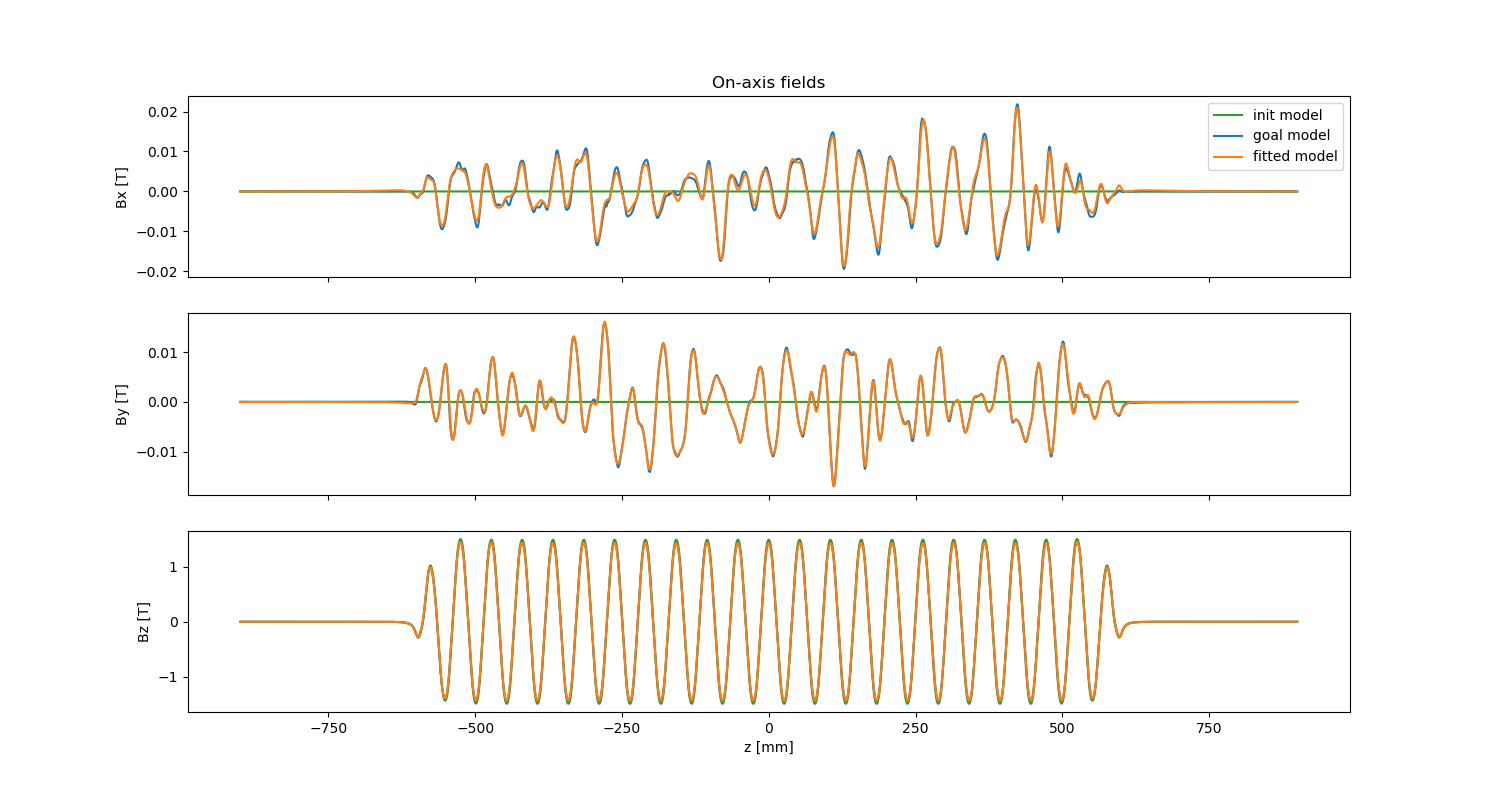
\includegraphics[width=.9\textwidth]{figures/field_fitting.png}
        \caption{Comparação entre campo medido pelo sensor hall e campo fornecido pelo modelo RADIA.}
        \label{fig:field_fitting}
    \end{figure}
\end{frame}


\section{References}

% Adding the option 'allowframebreaks' allows the contents of the slide to be expanded in more than one slide.
% \begin{frame}[allowframebreaks]{References}
% 	\tiny\bibliography{2023-10-06/references}
% 	\bibliographystyle{apalike}
% \end{frame}

\end{document}
